\documentclass[11pt]{scrartcl}
\usepackage[sexy]{evan}

\begin{document}
\title{AM 220 HW 1}
\author{Haozhe (Stephen) Yang}
\date{\today}
\maketitle

\section{Problem 1}

\begin{enumerate}[(a)]
    \item (i) As shown in the Jupyter notebook, the SVD decomposition of the rating matrix as $U \cdot \Sigma \cdot V^\top$. The python script prints out the matrices $U$ and $V^\top$, $\Sigma$ is a diagonal matrix with diagonal elements as \[14.16414875,\, 10.57294154, \, 3.24818406, \, 2.30083032, \, 1.79585698, \, 0.7212317 \]
    
    (ii) From the Singular Value Decomposition (SVD), we obtain six singular values. Retaining $k=2$ singular values provides a good balance, it captures the majority of the variance in the data while simplifying interpretation. The rankings and clustering remain stable, meaning most of the important information is retained. This is also shown in the Jupyter notebook, where we either keep two or three of the singular values.

    (iii) We can group movies by Genre. The first Genre is Sci-Fi, which includes Matrix, Star Wars, and Jurassic Park. The other three movies are Romance movies, which includes Titanic, La La Land, and Amelie. We can see from the ratings in the decomposition that the first vector favors Sci-Fi movies and the second second vector favors Romance movies. As a result, the SVD decomposition keeping two singular values shrinks down the movie space based on genre.
    \item (i) We project Henry onto the subspace spanned by our two vectors, and end up with $(-2.60, -0.65)$. We see that from the outputs, the Sci-Fi movies has a large negative score on the first component, and romance movies has a large positive score on the second component, and as a result, based on Henry's projection, we see that Henry likes Sci-Fi, and hence we should recommend Sci-Fi movies to Henry.
    
    (ii) We should recommend Matrix, Star Wars, and Jurassic Park to Henry, in the Sci-Fi category.
\end{enumerate}

\newpage

\section{Problem 2}

\begin{enumerate}[(a)]
    \item Note that $D$ is the degree matrix of the ring. Each vertex has degree 2, so $D$ is $2I$. Moreover, we see that $A$ is defined at the beginning of the problem, so we see that:
    \[I - D^{-1/2}AD^{-1/2} = \left[\begin{array}{cccccccc}
        1 & -\frac 14 & 0 & 0 & \dots & 0 & -\frac 14 \\
        -\frac 14 & 1 & -\frac 14 & 0 & \dots & 0 & 0 \\
        0 & -\frac 14 & 1 & -\frac 14 & \dots & 0 & 0 \\
        0 & 0 & -\frac 14 & 1 & \dots & 0 & 0 \\
        \vdots & \vdots & \vdots & \vdots & \ddots & \vdots &\vdots \\
        0 & 0 & 0 & 0 &\dots & 1 & -\frac 14 \\
        -\frac 14 & 0 & 0 & 0 &\dots & -\frac 14 & 1 \\
    \end{array}\right]\]
    In particular, we see that this is a circulant matrix. Moreover, we see that the $D^{-1/2}AD^{-1/2}$ just the diagonal above and below the main diagonal as $\frac 14$. Therefore, we see that the eigenvectors of $D^{-1/2}AD^{-1/2}$ are exactly \[\mathbf v_k = (1 \; \omega^k \; \omega^{2k} \; \dots \; \omega^{(N-1)k})\]
    where $k = 0, 1, \dots, N-1$ and $\omega$ is the primitive root of unity of the equation $X^N=1$. In particular, each has eigenvalue $\frac{1}{2}\cos\left(\frac{2\pi k}{N}\right)$.

    As such, we see that for the matrix $I-D^{1/2}AD^{-1/2}$, we have that the eigenvalues are still these vectors, but the eigenvalues for $\mathbf v_k$ is $\lambda_k = 1-\frac 12\cos(\frac{2\pi k}{N})$ for $k=0, 1, \dots, N-1$.
    \item Note that because $A$ is exactly $2 \cdot D^{-1/2}AD^{-1/2}$. Then we see that $A$ has eigenvectors still $\mathbf v_k$, but the corresponding eigenvalues are $\cos\left(\frac{2\pi k}{N}\right)$. Therefore, we have that $I-A$ has the eigenvectors $\mathbf v_k$ and eigenvalues $1-\cos\left(\frac{2\pi k}{N}\right)$.
    
    Moreover, because $(I-A)^\top = I-A$, so we see that the eigenvectors of $(I-A)^\top(I-A)$ are still $\mathbf v_k$ each with eigenvalue $\left[1-\cos\left(\frac{2\pi k}{N}\right)\right]^2$. We have previously denoted the eigenvectors as $\lambda_k$, so for $(I-A)^\top(I-A)$, the eigenvalues for $\mathbf v_k$ is $(2\lambda_k - 1)^2$.
    \item In diffusion maps, the embedding is constructed using the top few nontrivial eigenvectors of \( P^t \) (for some \( t>0 \)). Here, the eigenvectors remain unchanged, while their eigenvalues become \( \lambda_k^t \). 

    For a two-dimensional embedding, we just take the real and imaginary parts of \( v_1 \), yielding:
    \[
    x_n = \cos \left( \frac{2\pi n}{N} \right), \quad
    y_n = \sin \left( \frac{2\pi n}{N} \right), \quad
    n=0,\dots,N-1.
    \]
    These points \( (x_n, y_n) \) lie on the unit circle in \( \mathbb{R}^2 \).
    Therefore, we see that the vertices will be places equally spaced on the unit circle.

    In particular, this gives a very good embedding since the resulting embedding gives the exact structure of the $N$-ring. The original \( N \)-ring is already a one-dimensional manifold. Embedding it in \( \mathbb{R}^2 \) as a perfect circle is a very natural representation.
\end{enumerate}

\newpage

\section{Problem 3}

\begin{enumerate}[(a)]
    \item We first evaluate the integral \[\int_0^{2\pi} \Delta^2(\theta_i, \phi) d\phi\]
    WLOG, we assume that $\theta_i \le \pi$. This is because for any $\theta_i$, we can just do $\theta_i' = 2\pi - \theta_i$ and we have that $\Delta(\phi, \theta_i) = \Delta(2\pi - \phi, \theta_i')$, and so \[\int_0^{2\pi} \Delta^2(\theta_i, \phi) d\phi = \int_0^{2\pi} \Delta^2(2\pi-\phi, \theta_i') d\phi = \int_0^{2\pi} \Delta^2(\phi, \theta_i')d\phi \]
    
    Therefore, we assume $\theta_i \le \pi$, since otherwise we just take $\theta_i'$ to evaluate the integral. Note that $\Delta^2(\phi, \theta_i) = (\phi-\theta_i)^2$ for $\theta_i \in [0, \pi+\theta_i]$. And $\Delta^2(\theta_i, \phi) = [2\pi - (\phi - \theta_i)]^2$. So we can break down the integral into
    \begin{align*}
        \int_0^{2\pi} \Delta^2(\theta_i,\phi) \, d\phi &= \int_0^{\theta_i+\pi} (\phi-\theta_i)^2 \, d\phi + \int_{\theta_i+\pi}^{2\pi} [2\pi - (\phi - \theta_i)]^2 \, d\phi \\
        &= \left[\frac 13(\phi-\theta_i)^3\right]_0^{\theta_i + \pi} + \left[\frac 13 (\phi - 2\pi - \theta_i)^3\right]_{\theta_i+\pi}^{2\pi} \\
        &= \frac 13 \left(\pi^3 + \theta_i^3 - \theta_i^3 + \pi^3 \right) \\
        &= \frac{2\pi^3}{3}
    \end{align*}
    
    Note that we have found \[\int_0^{2\pi} \Delta^2(\theta_i, \phi) d\phi = \frac{2\pi^3}{3}\]
    for any value of $\theta_i$. Therefore, we evaluate the original integral and we find that \begin{align*}
        & g(\theta_i, \theta_j) \\
        =& \frac{1}{2} \left[ \int_0^{2\pi} \frac{d\phi}{2\pi} \left( \triangle^2 (\theta_i, \phi) + \triangle^2 (\phi, \theta_j) \right) - \int_0^{2\pi} \frac{d\phi}{2\pi} \int_0^{2\pi} \frac{d\psi}{2\pi} \triangle^2 (\phi, \psi) - \triangle^2 (\theta_i, \theta_j) \right] \\
        =& \frac{1}{2} \left[ \int_0^{2\pi} \frac{d\phi}{2\pi} \triangle^2 (\theta_i, \phi) + \int_0^{2\pi} \frac{d\phi}{2\pi} \triangle^2 (\theta_j, \phi) - \int_0^{2\pi} \frac{d\phi}{2\pi} \cdot \frac{1}{2\pi} \int_0^{2\pi} \triangle^2 (\phi, \psi) d\psi - \triangle^2 (\theta_i, \theta_j) \right] \\
        =& \frac 12 \left[\frac{1}{2\pi} \cdot \frac{2\pi^3}{3} + \frac{1}{2\pi} \cdot \frac{2\pi^3}{3} - \int_0^{2\pi} \frac{d\phi}{2\pi} \cdot \frac{1}{2\pi} \cdot \frac{2\pi^3}{3} - \Delta^2(\theta_i, \theta_j)\right] \\
        =& \frac 12\left[\frac{2\pi^2}{3} - \frac{\pi}{6} \cdot 2\pi - \Delta^2(\theta_i, \theta_j)\right] \\
        =& \frac{\pi^2}{6} - \frac 12\Delta^2(\theta_i, \theta_j)
    \end{align*}
    \item We see the following plot in Desmos: \begin{center}
        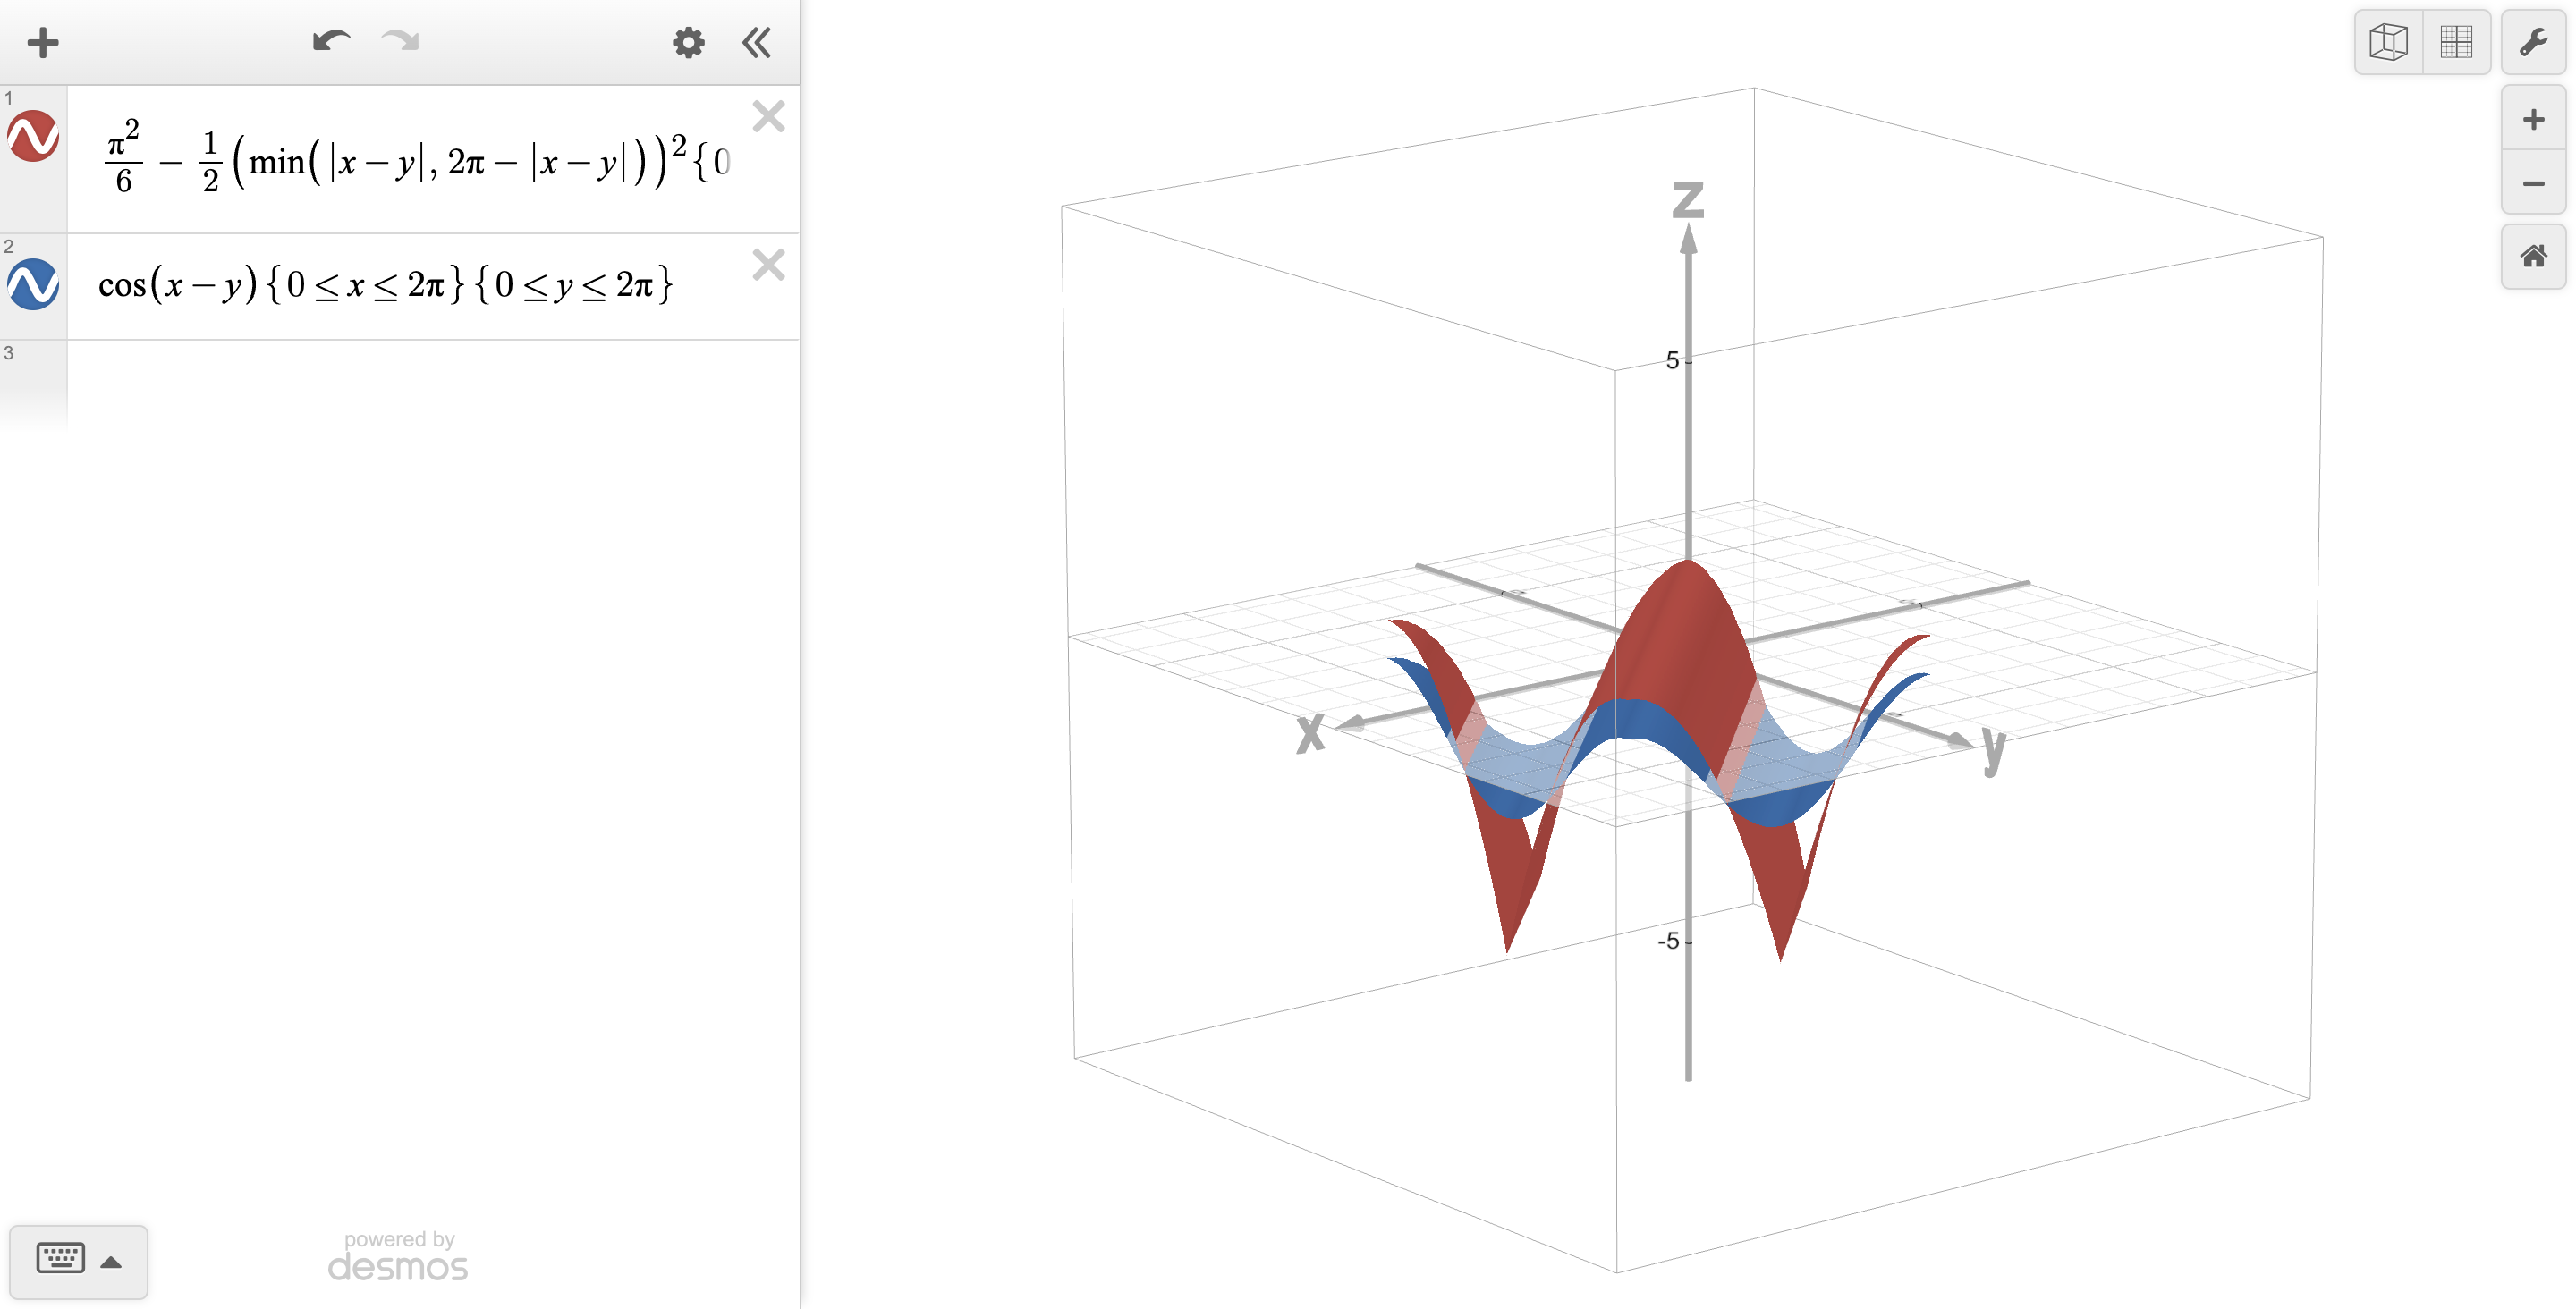
\includegraphics[width = 13cm]{hw1-img/hw1-p3.png}
    \end{center}
    The red plot is our function, and the blue plot is the inner product. A key observation is that these two functions closely approximate each other, particularly when the differences in $x$ and $y$ are small. This means that the local distances in Euclidean space are well-aligned with the corresponding distances when expressed in polar coordinates. In particular, the local structure of the data is preserved across different representations, reinforcing the robustness of techniques that rely on distance-based relationships, such as Isomap.
\end{enumerate}

\newpage

\section{Problem 4}

We can first plot the two data sets in 3D, here are the plots: \begin{center}
    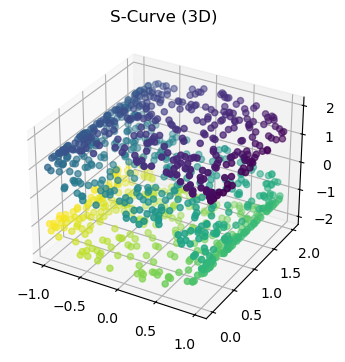
\includegraphics[width=7cm]{hw1-img/hw1-p4-1.png}
    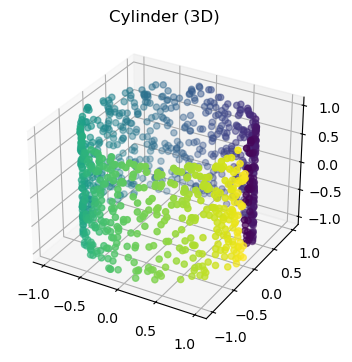
\includegraphics[width=7cm]{hw1-img/hw1-p4-2.png}
\end{center}
Then we run the three algorithms on these two datasets and get the following results: \begin{center}
    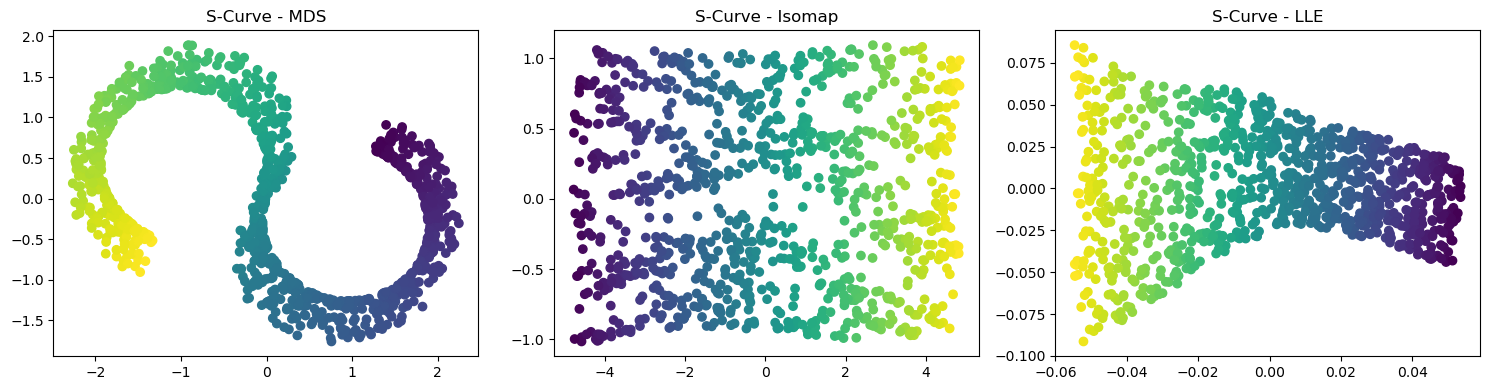
\includegraphics[width=14cm]{hw1-img/hw1-p4-3.png}
    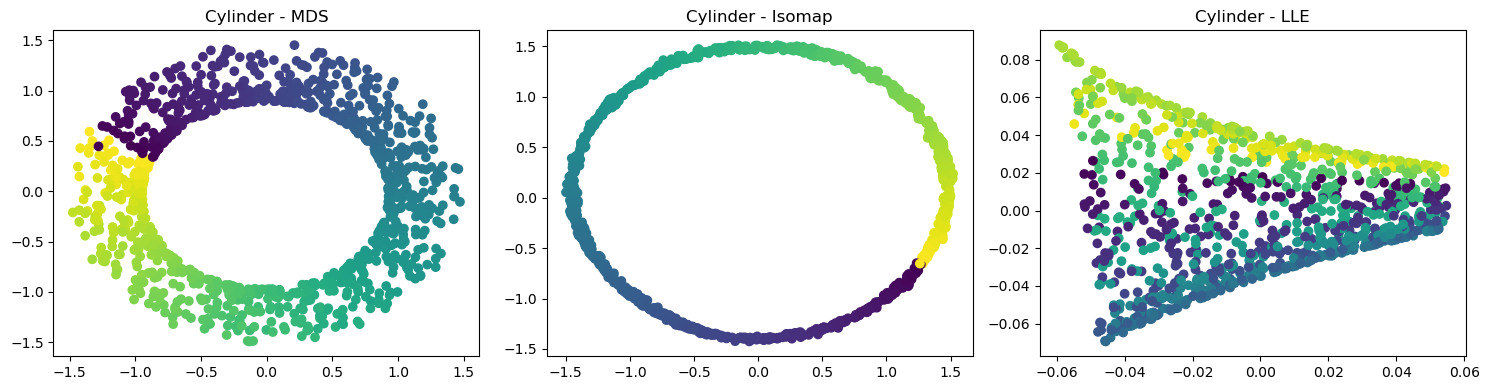
\includegraphics[width=14cm]{hw1-img/hw1-p4-4.png}
\end{center}

Here are the observations of the Three Learned Manifolds

\paragraph{S-Curve Dataset}
\begin{itemize}
    \item MDS: The MDS projection of the S-Curve successfully captures its global structure, unfolding it into an ``S''-shaped representation. The relative distances between points remain preserved, making it a useful approach for maintaining global distances.
    \item Isomap: Isomap unfolds the S-Curve into a more linear form, preserving geodesic distances better than MDS. The overall structure is flattened into a nearly rectangular shape, suggesting that Isomap effectively represents the intrinsic geometry of the manifold.
    \item LLE: LLE produces a more localized representation. The output appears compressed and somewhat distorted compared to Isomap and MDS. It is evident that LLE emphasizes local relationships between points but fails to fully capture the global structure of the S-Curve.
\end{itemize}

\paragraph{Cylinder Dataset}

\begin{itemize}
    \item MDS: MDS projects the cylindrical manifold into a circular structure, effectively preserving its global shape. The arrangement of points follows the expected cylindrical unfolding, maintaining relative distances.
    \item Isomap: Isomap performs similarly to MDS, representing the cylindrical data as a well-formed circular structure. This suggests that Isomap successfully captures both local and global geometric properties of the cylinder.
    \item LLE: LLE results in a compressed and distorted representation, similar to what was observed with the S-Curve. While it maintains some locality, it does not retain the cylindrical shape effectively. The unfolding is stretched in a way that does not correspond to the expected global structure.
\end{itemize}

\paragraph{Best Preforming Algorithms}

\begin{itemize}
    \item Isomap appears to perform best overall, as it successfully unfolds both the S-Curve and Cylinder while preserving their intrinsic geometry. Its ability to approximate geodesic distances leads to more accurate low-dimensional embeddings.
    \item MDS is a close second, as it effectively maintains global structure but does not necessarily account for geodesic distances as well as Isomap.
    \item LLE performs the worst, as it prioritizes local relationships at the cost of global structure. The learned manifolds appear distorted and fail to retain the expected large-scale geometric properties.
\end{itemize}

The $Q$ scores accurately reflect this:

\begin{verbatim}
S-Curve Dataset
MDS    | Local Q-score = 0.462, Global Q-score = 0.964
Isomap | Local Q-score = 0.849, Global Q-score = 0.902
LLE    | Local Q-score = 0.596, Global Q-score = 0.743

Cylinder Dataset
MDS    | Local Q-score = 0.497, Global Q-score = 0.889
Isomap | Local Q-score = 0.196, Global Q-score = 0.870
LLE    | Local Q-score = 0.425, Global Q-score = 0.629
\end{verbatim}

The Q-scores further validate these findings, as Isomap achieves the highest Local Q-score, and a very high Global Q-score for the S-Curve. MDS excels in maintaining global relationships, as seen in its highest Global Q-scores for both the S-curve and cylinder, though its local preservation is weaker. LLE consistently scores the lowest across both datasets, with Global Q-scores of 0.743 and 0.629, confirming that it sacrifices global structure for local relationships but does not outperform Isomap or MDS in either metric.

\newpage

\section{Problem 5}

We plot the two datasets as \begin{center}
    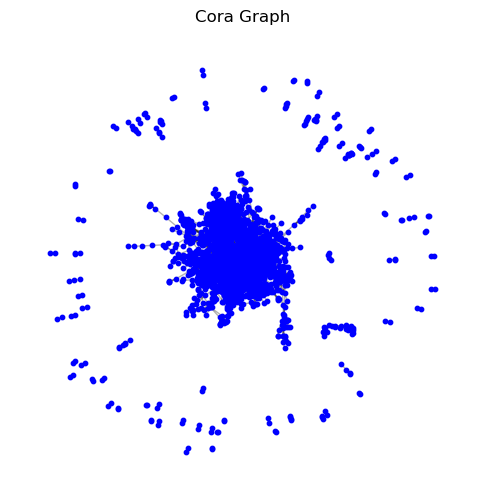
\includegraphics[width=6cm]{hw1-img/hw1-p5-1.png}
    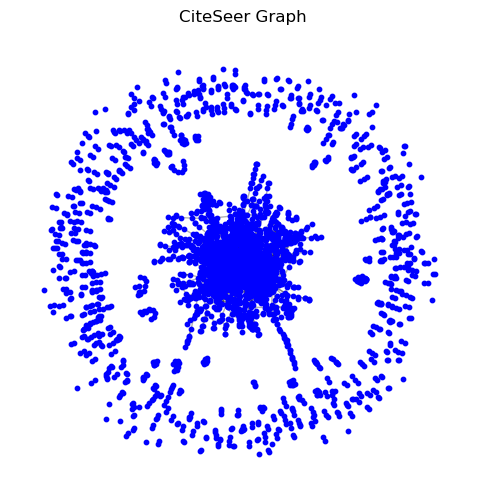
\includegraphics[width=6cm]{hw1-img/hw1-p5-2.png}
\end{center}
We also plot the resulting representations: \begin{center}
    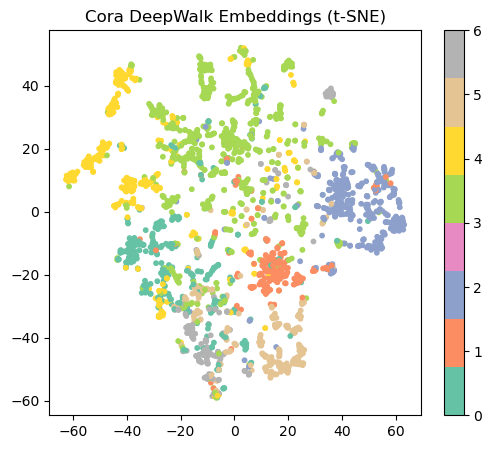
\includegraphics[width=4.5cm]{hw1-img/hw1-p5-3.png}
    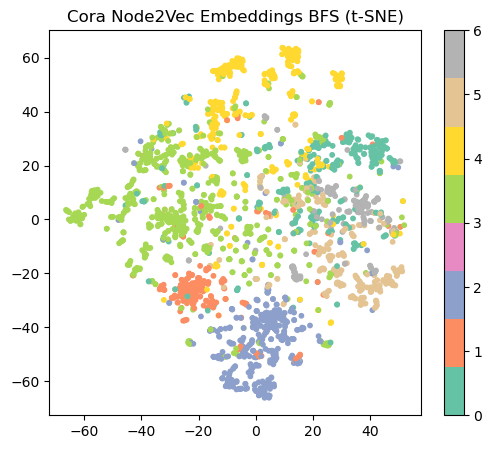
\includegraphics[width=4.5cm]{hw1-img/hw1-p5-4.png}
    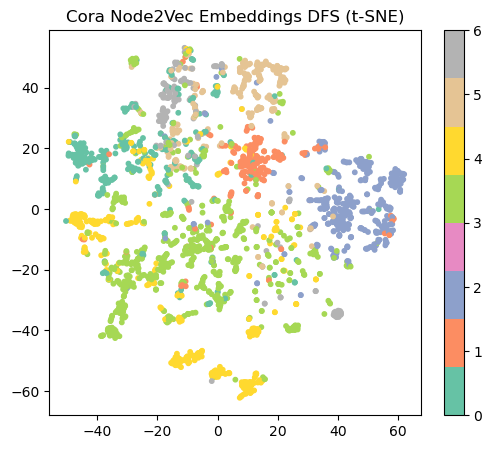
\includegraphics[width=4.5cm]{hw1-img/hw1-p5-5.png}
\end{center}
\begin{center}
    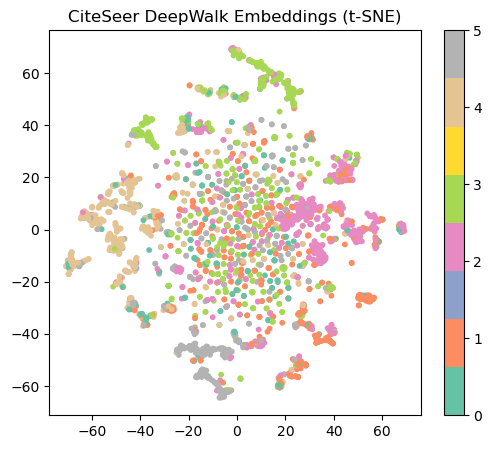
\includegraphics[width=4.5cm]{hw1-img/hw1-p5-6.png}
    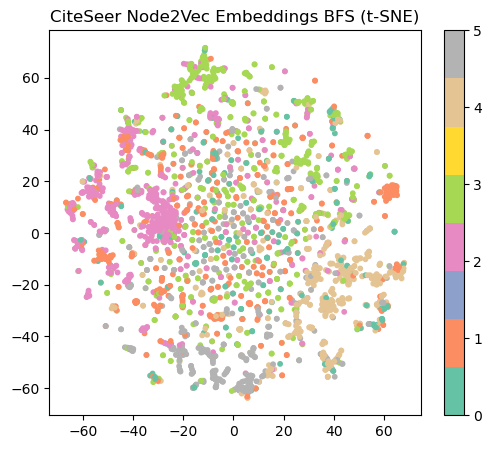
\includegraphics[width=4.5cm]{hw1-img/hw1-p5-7.png}
    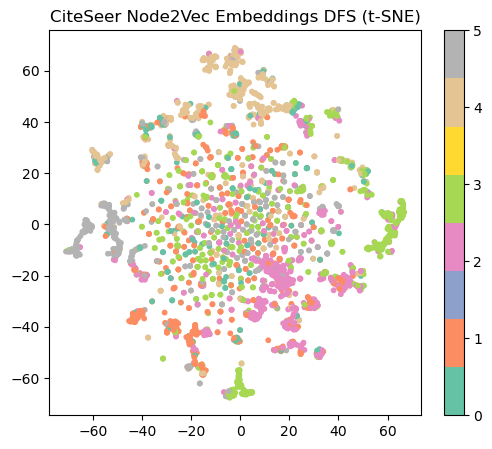
\includegraphics[width=4.5cm]{hw1-img/hw1-p5-8.png}
\end{center}

We visualize the Cora and CiteSeer datasets and their learned representations using DeepWalk and Node2Vec (with BFS and DFS sampling). The Cora embeddings show distinct clusters that align well with the dataset's six categories. Meanwhile, CiteSeer embeddings are more scattered, making it harder to distinguish clusters. Even so, regardless of whether BFS, DFS, or DeepWalk is used, the learned representations look quite similar, suggesting that the embedding methods capture comparable structural patterns in both datasets.

To measure embedding quality, we test them on node classification:

\begin{verbatim}
    Cora Classification Accuracy
    DeepWalk: Val = 70.4%, Test = 71.7%
    Node2Vec (BFS): Val = 61.0%, Test = 63.1%
    Node2Vec (DFS): Val = 69.4%, Test = 73.1%

    CiteSeer Classification Accuracy
    DeepWalk: Val = 47.6%, Test = 48.3%
    Node2Vec (BFS): Val = 40.4%, Test = 39.0%
    Node2Vec (DFS): Val = 50.4%, Test = 48.4%
\end{verbatim}

DeepWalk and Node2Vec (DFS) consistently outperform BFS, suggesting that DFS captures more useful structural information for classification. Cora, with its well-defined clusters, benefits the most from these methods, while CiteSeer remains harder to classify. More training time or optimized walk strategies could further improve performance. With more training, CiteSeer's embeddings could improve as longer or more frequent walks better capture its structure. Since loss was still decreasing, additional iterations or tuning walk parameters could enhance separation and boost classification accuracy.

\end{document}